% !TEX root = tracking.tex
\section{Introduction}
 Currently there is great interest both in research and industry to find methods of fast motion planning for unmanned aerial vehicles (UAVs) and other autonomous systems. These systems must be able to plan and execute a dynamic trajectory in real-time without violating safety constraints. This is a very difficult challenge: the need for fast planning is generally at odds with the need for maintaining safety and robustness. In order to achieve real-time planning for any environment with static obstacles, researchers typically use highly simplified model dynamics or kinematics, resulting in a tracking error between the planned path and the true high-dimensional system. This concept is illustrated in Fig. \ref{fig:chasing}, where the path was planned using a simplified planning model, but the real vehicle cannot track this path exactly. In addition, most current planners do not consider the possible effect of external disturbances (e.g. wind) on the system. The tracking error that arises due to modeling with simplified dynamics and lack of disturbances can lead to unsafe situations in which the planned path may be safe, but the actual system trajectory violates unsafe regions.

We propose a modular tool FaSTrackHD: Fast and Safe Tracking for High Dimensional systems, which works by modeling the navigation task as a sophisticated tracking system following a simplified planning system. Offline, a precomputed capture-avoid game between the two systems is analyzed using Hamilton Jacobi (HJ) reachability analysis. This results in a \textit{tracking error function} that maps the initial relative state between the two systems to the maximum possible relative distance that occurs over time (i.e. the tracking error bound), accounting for bounded worst-case external disturbances. This tracking error bound can be thought of as a ``safety bubble" around the planning system. The precomputation also provides a \textit{safety control function} that will map the current relative state to the optimal safety control for the tracking system to ``catch" the planning system. It is important to note that the offline computations are \textit{independent} of the path planned in real-time; what matters are the relative states and dynamics between the systems, not the absolute state of the online path.

In the online computation, the tracking error bound is determined by the initial relative state between the planning and tracking systems. The sensed obstacles are augmented by this bound to ensure that no potentially unsafe paths can be computed. Next a path or trajectory planner uses the simplified planning model to determine the next desired state. The tracking system then finds the relative state between itself and the next desired state. If this relative state is nearing the tracking error bound then it is plugged into the safety control function to find the instantaneous optimal safety control of the tracking system. This process is repeated until the navigation goal is reached. 
  

\begin{figure}
	\centering
	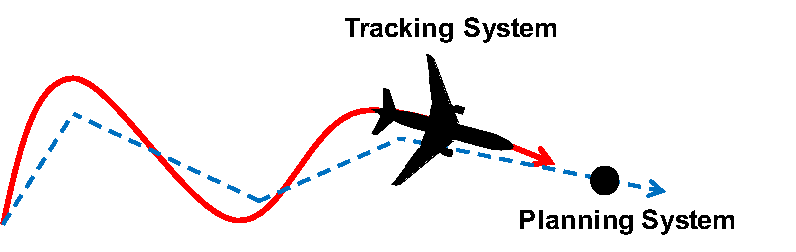
\includegraphics[width=0.4\textwidth]{fig/chasing}
	\caption{A planning system using a fast but simple model, followed by a tracking system using a dynamic model}
	\label{fig:chasing}
	\vspace{-.2in}
\end{figure}
%
FASTrack is designed to be modular and able to use in conjunction with various fast path and trajectory planners to add robustness and safety guarantees. In this paper we demonstrate this tool by computing a capture-avoid game between a 10D quadrotor model and a linear 3D constant-velocity model. We then plan a path using rapidly-exploring random trees (RRT) through an environment with wind and static obstacles. \textcolor{red}{state results}